\documentclass{article}
\usepackage{graphicx}
\usepackage{amsmath}

\title{Introduction to Machine Learning Assignment 2}
\author{Divij Singh}
\date{18/09/18}


\begin{document}

	\maketitle
	
	\section{Q1}
	(a) \\ \\$e^x = \sum_{n=0}^{\infty} \frac{x^n}{n!} = 1 + x +\frac{x^2}{2!} ...$ (this is technically the Maclaurin expansion, which is a subest of Taylor series at a=0)\\ \\
(b)\\
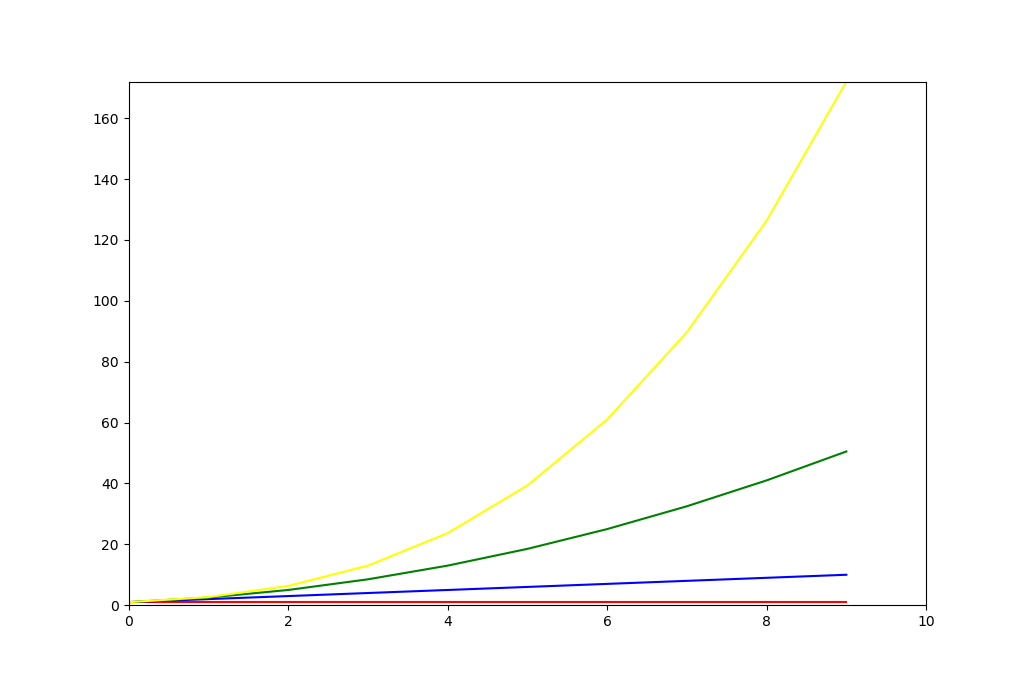
\includegraphics[scale=0.5]{taylor graph.png}

	
\section{Q2}
(a)
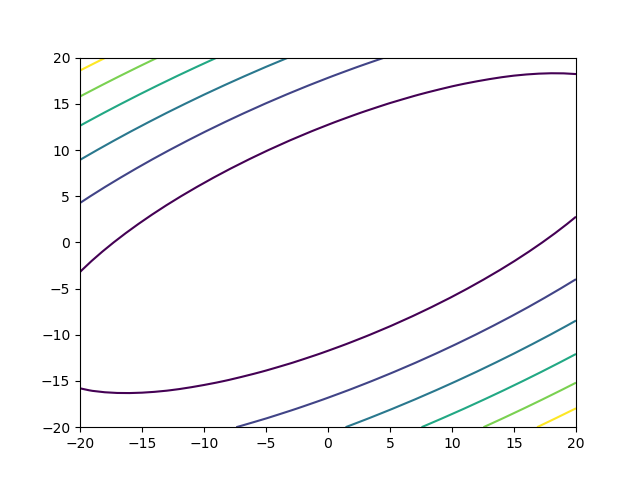
\includegraphics[scale=0.75]{contour map.png}\\ \\
(b)\\
\\
We differentiate $J(w) = \frac{1}{2}[(w_2 - w_1 )^2 + (1- w_1)^2]$ by both $w_1$ and $w_2$, to get $\frac{\partial J}{\partial w_1} = 2w_1 - w_2 -1$ and $\frac{\partial J}{\partial w_2} = w_2 - w_1$ giving us our gradient vector $\nabla(w)= \begin{bmatrix}2w_1 - w_2 -1 \\ w_2 - w_1 \end{bmatrix}$.\\
\\
(c)\\ \\
1. $\nabla(w)= \begin{bmatrix}2w_1 - w_2 -1= 21.19 \\ w_2 - w_1=-2.19 \end{bmatrix}$ where $x=20,y=17.81$\\ \\
2. $\nabla(w)= \begin{bmatrix}2w_1 - w_2 -1= -25.25 \\ w_2 - w_1=4.25 \end{bmatrix}$ where $x= -20, y= -15.75$\\ \\
3. $\nabla(w)= \begin{bmatrix}2w_1 - w_2 -1= -5.57  \\ w_2 - w_1=-5.43 \end{bmatrix}$ where $x=-10,y=-15.43$\\ \\
\\
(d)\\ \\
We need values such that $2w_1 - w_2 -1 = 0$ and $w_2 - w_1 = 0$\\
From the second equation, we get $w_2=w_1$, giving us $w_1=1$ (which means that $w_2 = 1$)

\section{Q3}

\end{document}